\section{Differentially Private Traffic Shaping}
\label{sec:dp}

\if 0
\begin{algorithm}[t]
    \DontPrintSemicolon
    \SetNoFillComment
    % \KwIn{$S_N, Q, T, \varepsilon, w, D, min\_burstsize, max\_burstsize$}
    \SetKwFunction{get}{get\_dp\_size}
    \SetKwFunction{send}{send\_data}
    \SetKwFunction{dequeue}{dequeue}
    \SetKwFunction{doshape}{do\_shape}
    \SetKwFunction{addhdr}{add\_dp\_header}
    \SetKwFunction{encrypt}{encrypt}
    \SetKwFunction{sendpkt}{send\_udp\_pkt}
    \SetKwProg{Fn}{Function}{:}{}

    \Fn{\get{$Q,\; \varepsilon$}}{
        \am{where do $D_N$, $B_{min}$, $B_{max}$ come from?} \;
        $D^N = Q + \mathcal{N}(0, \sigma)$ \;
        $D^{N}_{clipped} =\max (B_{min}, \; \min (B_{max}, \; D_N))$ \;
        \textbf{return} $D^{N}_{clipped}$ \;
    }
    \Fn{\send{$len_R,\; len_D,\; MTU$}}{
        buf[0:$len_R$ -1] = \dequeue($Q_R$, $len_R$)\;
        buf[$len_R$:$len_R$ + $len_D$ -1] = \dequeue($Q_D$, $len_D$)\;
        \While{(buf.size $\neq$ 0)}{
            plen = buf.size > MTU ? MTU : buf.size\;
            pkt.payload = buf.get\_data(plen)\;
            buf.size -= sizeof(pkt.payload)\;
            \tcc{Header to track dummy data.}
            pkt.payload = \addhdr(pkt.payload)\;
            pkt.payload = \encrypt(pkt.payload)\;
            \sendpkt(pkt)\;
        }
    }
    \Fn{\doshape{}}{
        %\textbf{SendPacket}(queue\_state, pkt\_size, delay)\;
        \While{(not at end of data transmission)}{
            {sleep}($T$)\;
            $t$ = {get\_current\_time}()\;
            $Q_t$ = {get\_queue\_size}($t$)\;
            $D^S_t$ = \get($Q_t, \; \varepsilon$)\;
            $D^R_t$ = $\min (Q_t, D^S_t)$ \tcc{payload len}
            $D^P_t$ = $D^S_t - D^R_t$ \tcc{dummy len}
            \send$(D^R_t,\; D^P_t,\; MTU)$ \;
        }
    }
    \caption{Shaper logic}
    \label{alg:middle-box-all}
\end{algorithm}
\fi

% In this section, we describe our conceptual shaping strategy. In the next
% sections, we describe the design of our complete system that uses the strategy
% while shaping actual traffic.

Shaping involves transmitting packets such that their sizes and timing do not reveal secrets.
The goal of our DP traffic shaping mechanism is to dynamically adjust the data transmission rate based on the available data stream, all while ensuring that the DP guarantees hold for any information that an attacker, as defined in our threat model (\S\ref{subsec:threat-model}), can observe.
The design of our traffic shaping algorithm relies on three key steps.
%
First, we formalize the information available to an attacker observing an application stream, which is all information such as packet sizes or timing at the finest granularity of observation.
We propose to use a buffering queue to collapse all this information into a sufficient statistic to adapt {\sys}'s transmission rate: the size of data in the queue waiting to be transmitted through our shaping mechanism (\S\ref{subsec:infromation-bottleneck}).
%
Second, we show how to perform {\em DP measurements} of our buffering queue, in order to adapt \sys's transmission rate with DP guarantees.
Indeed, we show that under natural constraints on the transmission rate decision mechanism, the change of queue size is bounded, allowing us to perform DP measurements (\S\ref{subsec:dp-queue-measurements}).
%
Third, we describe our decision mechanism for sending data based on DP decisions, which completes our DP shaping mechanism (\Cref{alg:dp_shaping_mechanism}).
Intuitively, we can use DP queue measurements and public information such as network conditions to decide the amount of data to transmit.
Transmissions contain queued data when some is available, and dummy data otherwise.
The stream observed by any attacker is a post-processing of the DP queries issued on the queue (depends on the private data only through the DP measurements), and is hence DP.


% Our key insight is that the size of data waiting to be transmitted in our shaped
% tunnel is a sufficient statistic to adapt \sys's transmission rate.
% %
% by decapsulating \ml{?} packets and buffering content,
% we can make adaptive decisions on
% make adaptive decisions on this state, and only adapt to the data based on these measurements. We can then use the post-processing guarantee)
% We rely on periodic transmission intervals of constant lengths, while ensuring
% that the number of bytes transmitted within each interval is noised according to
% our differential privacy strategy.
% %
% The differentially private strategy relies on composition
% theorem~\citeme{dp-composition}. Specifically, we model an application
% stream as a sequence of windows of packet transmissions and reason
% about per-window linkage and accumulation of leakage over multiple
% windows.

% In the following, we provide a formal definition of differentially privacy in
% traffic shaping and then describe how we use it to shape application traffic
% streams.


% \label{subsec:infromation-bottleneck}
% \begin{figure}[t]
%   \centering
%   %  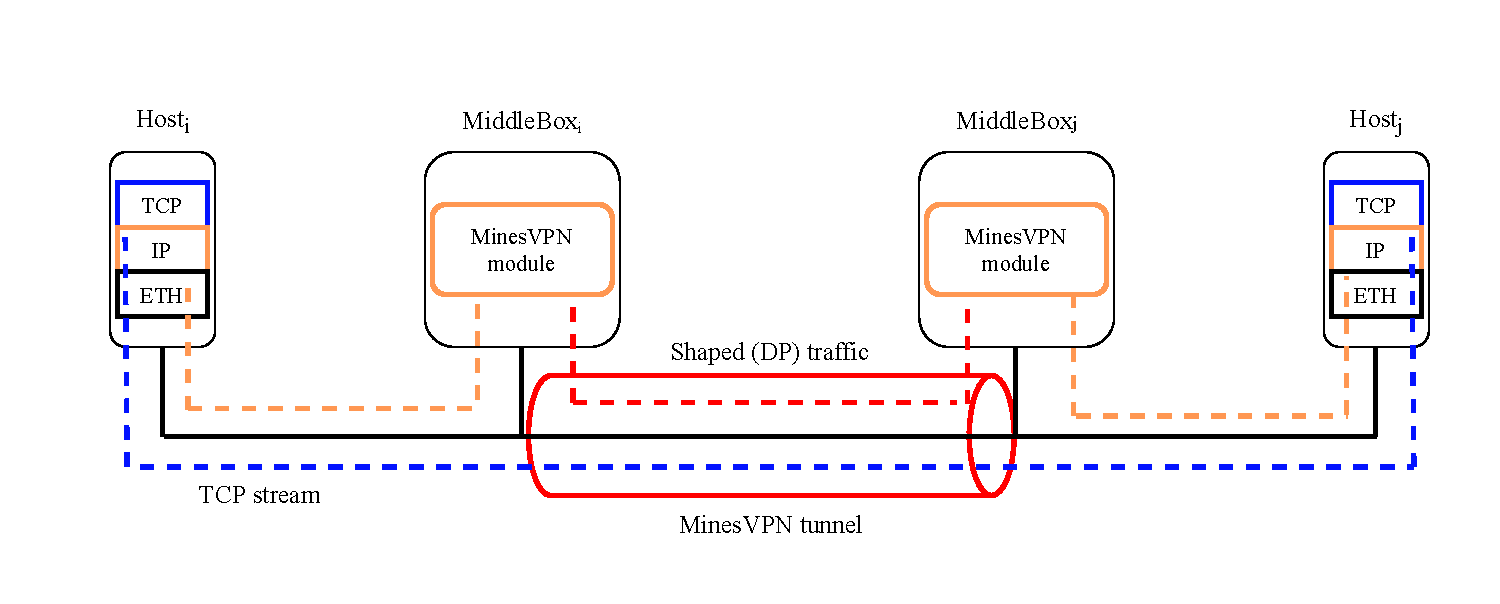
\includegraphics[width=\columnwidth]{figures/Design_highlevel.pdf}
%   %  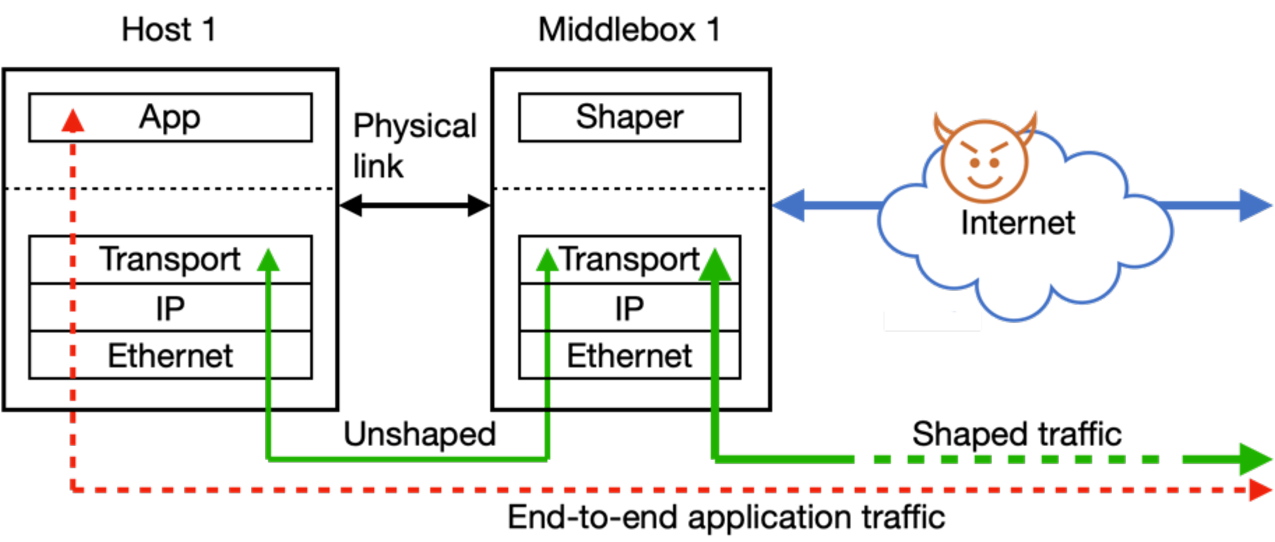
\includegraphics[width=\columnwidth]{figures/minesvpn-overview-half.pdf}
%   %  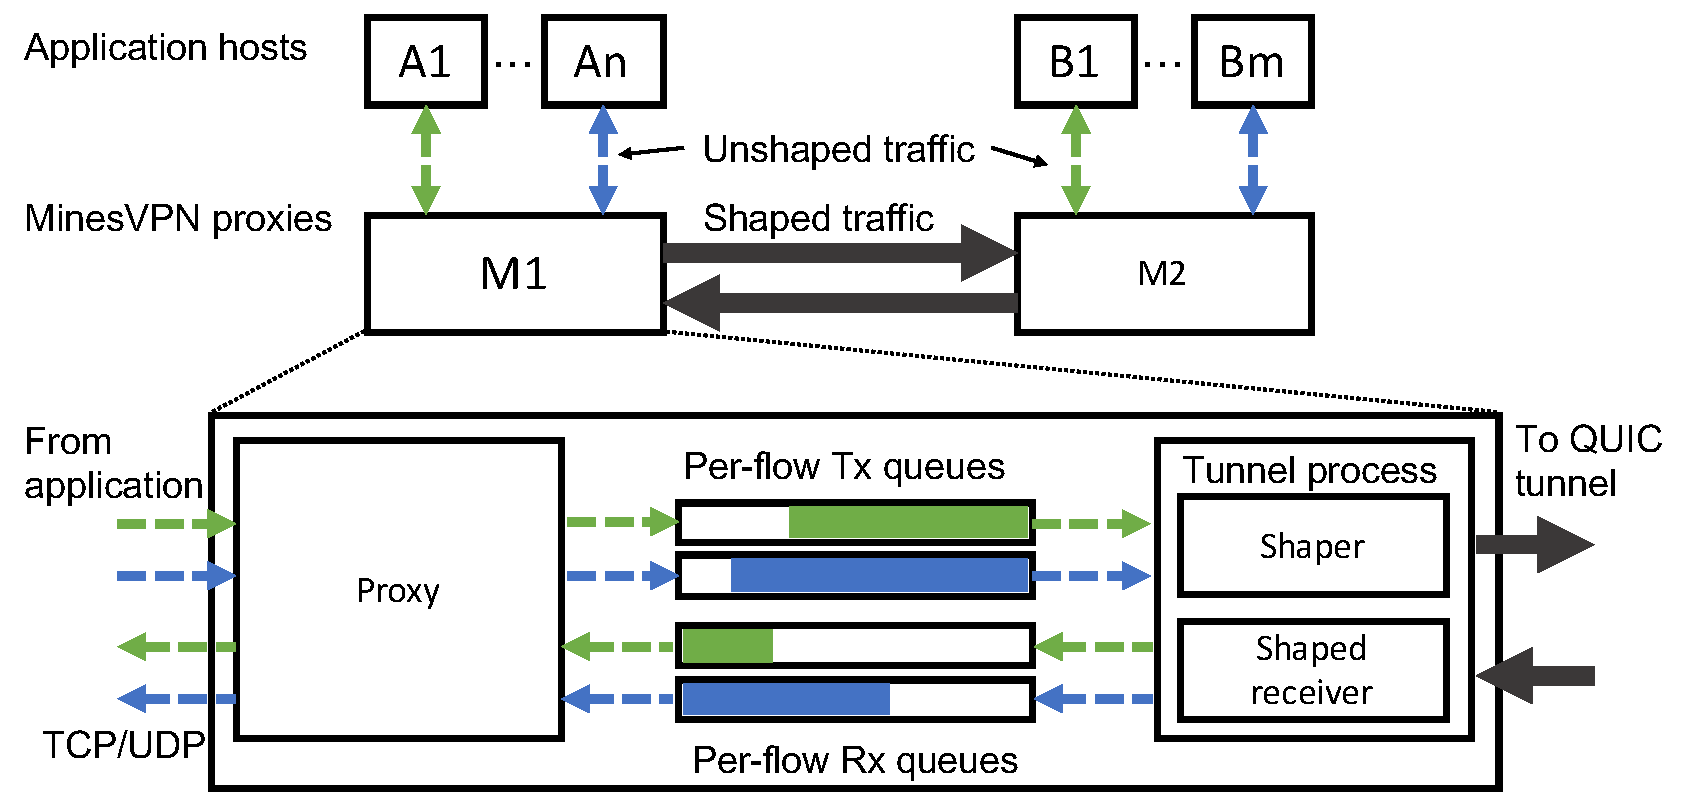
\includegraphics[width=\columnwidth]{figures/minesvpn-arch4.pdf}
%   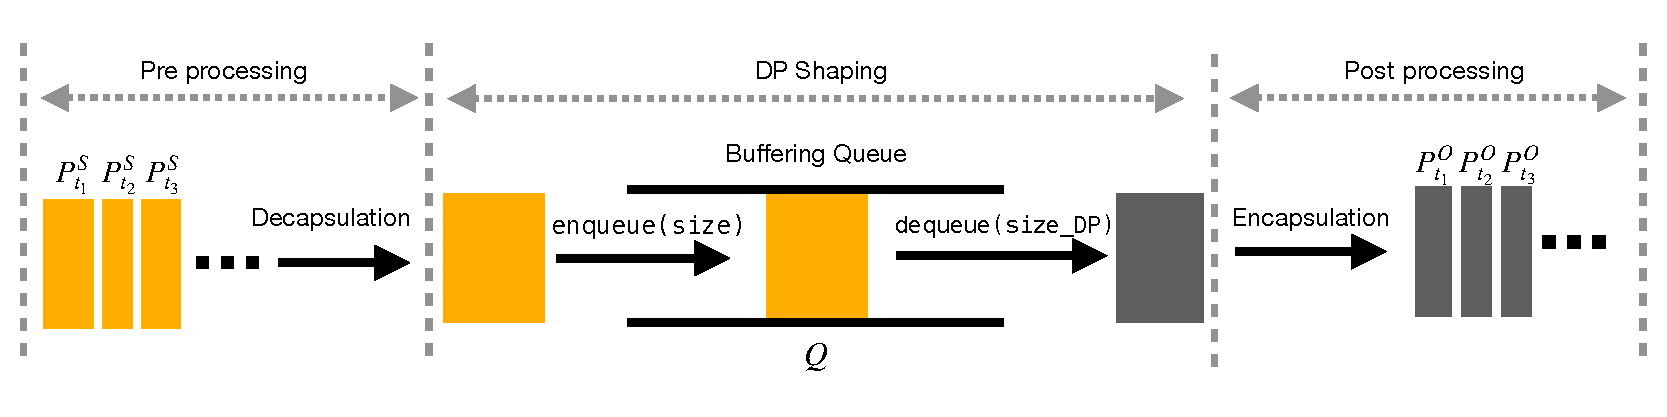
\includegraphics[width=\columnwidth]{figures/DPshaping_concept_horizontal.pdf}
%   \caption{{\sys} overview (one tunnel endpoint)
%       %\am{Update figure}
%   }
%   \label{fig:DPshaping_concept_horizontal}
% \end{figure}

\begin{figure}[t]
  \centering
  %  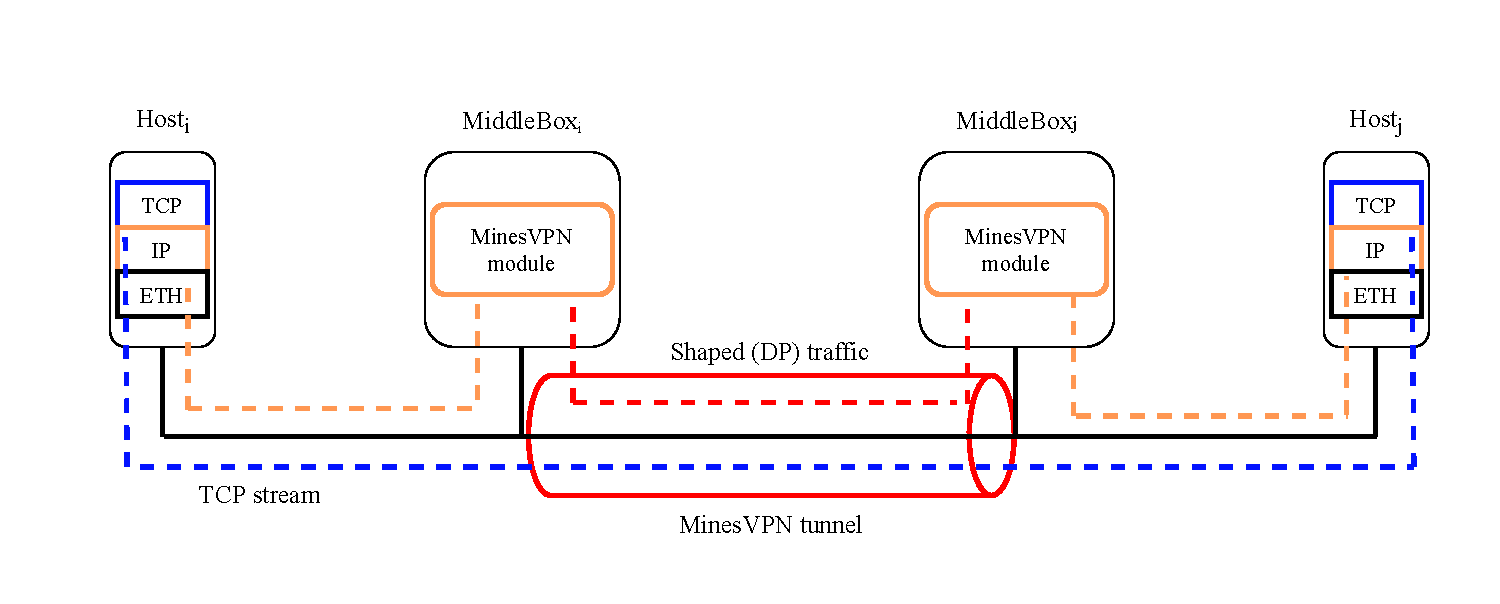
\includegraphics[width=\columnwidth]{figures/Design_highlevel.pdf}
  %  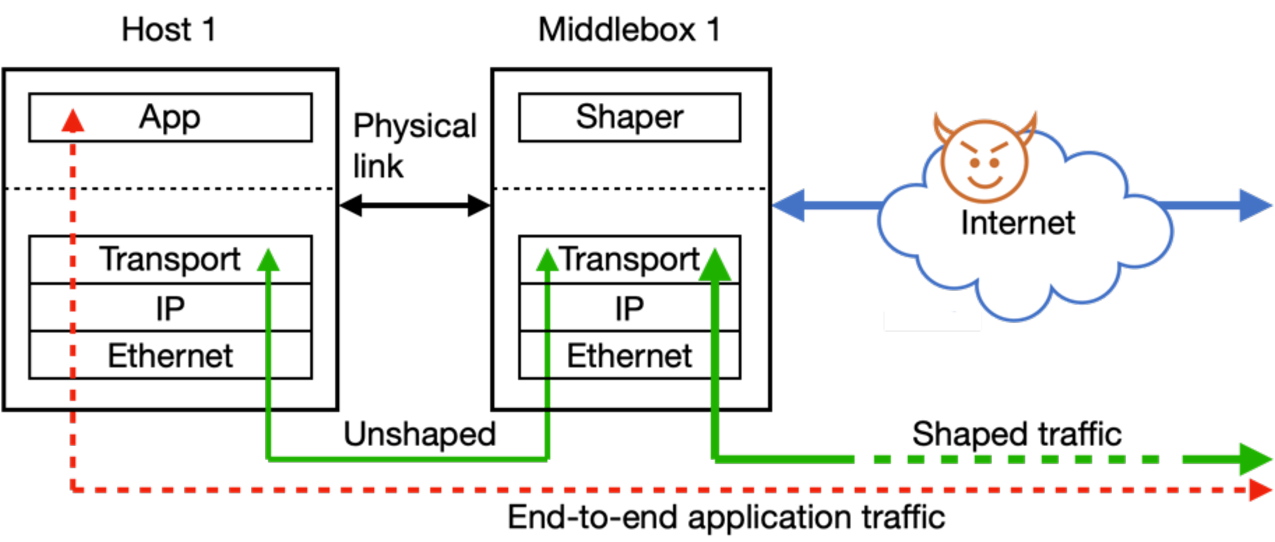
\includegraphics[width=\columnwidth]{figures/minesvpn-overview-half.pdf}
  %  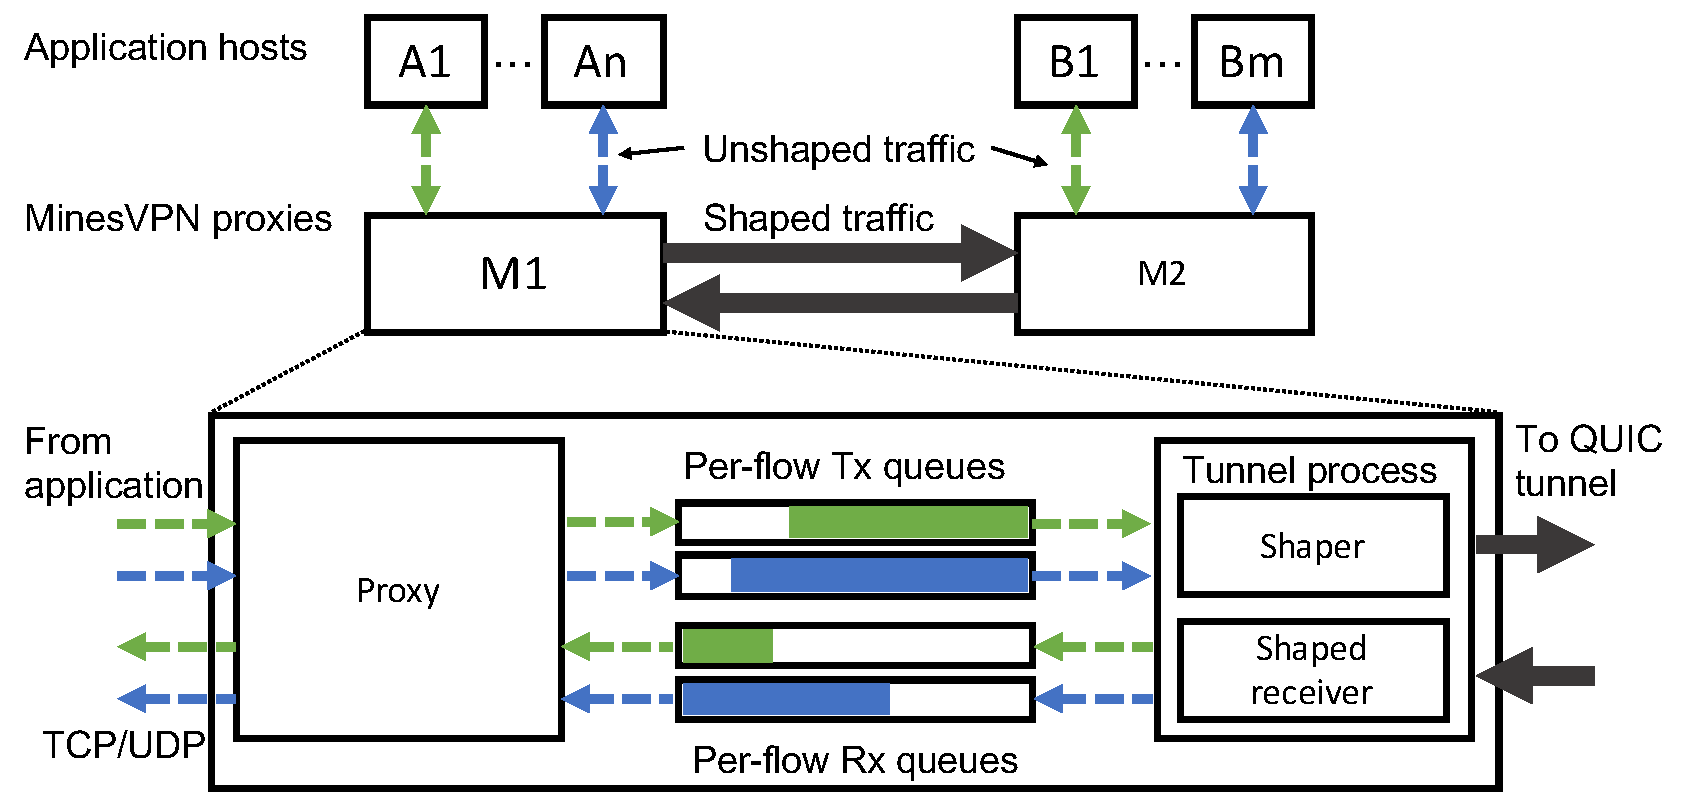
\includegraphics[width=\columnwidth]{figures/minesvpn-arch4.pdf}
  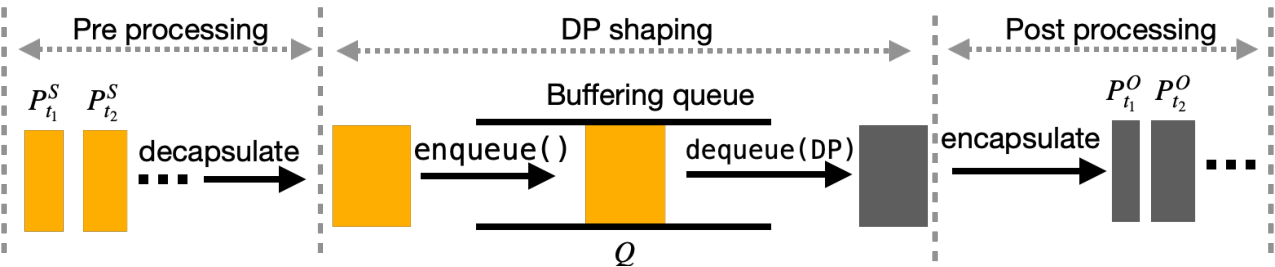
\includegraphics[width=\columnwidth]{figures/DPshaping_concept_vertical.pdf}
  \caption{{\sys} traffic shaping stages}
  \label{fig:DPshaping_concept_vertical}
\end{figure}

\subsection{DP shaping building blocks}
\label{subsec:infromation-bottleneck}
We define a source application stream $S$ (i.e. the input stream) as a sequence of packets:
\begin{equation}\label{equ:stream-pkts}
        S = \{P_{t_1}^S, P_{t_2}^S, P_{t_3}^S, \dots \} ,
\end{equation}
where $P_{t_i}^S$ is the size of the packet transmitted as a part of the stream
$S$ at the time $t_i$. \am{The symbol $S$ is overloaded in many places.}\as{all of them referring to the input stream}
%\am{I realize this model is inaccurate. A more accurate description is that an
%application byte stream is transformed into a sequence of packets. In absence of
%shaping, packet sizes and timing reveal the secrets. {\sys} transforms an {\em
%application byte stream} into a sequence of DP shaped bursts that are
%transmitted within fixed intervals. Basically, DP does not get an input as a
%packet stream but rather as a byte stream.}
%
Without {\sys}'s shaping, an eavesdropper can observe the entire stream:
$S = \{P_{t_1}^S, P_{t_2}^S, P_{t_3}^S, \dots \}$.
Typically, this information is strongly correlated with the data sent by the
application and the eavesdropper can infer sensitive information, such as the
specific video being sent by a streaming
application~\cite{schuster2017beautyburst}.


% We start by modeling an application stream in one direction as a
% dataset of packet sequences and by defining neighboring datasets from
% application streams.

% %\Cref{fig:minesvpn-arch} represents the abstracted design of the {\sys}
% %middle-box.  The incoming traffic in \Cref{fig:minesvpn-arch} is in form of
% %packets.  We formalize a stream of traffic, $S$, with the following
% %representation:

% %\smallksip\noindent
% \paragraph{Input stream.}
% We model an application stream, $S_I$ as a sequence of packets
% %$\{P_{t_1}^S, P_{t_2}^S, P_{t_3}^S, \dots \}$,

% \begin{equation}\label{equ:stream-pkts}
        % S_I = \{P_{t_1}^S, P_{t_2}^S, P_{t_3}^S, \dots \}
% \end{equation}
% where $P_{t_i}^S$ is the size of the packet transmitted as a part of the stream
% $S$ at the time $t_i$.

%leading to information leakage \cite{beautyburst} \todo{More
%references are needed}.
%{\sys}'s {\DPlogic} decides {\em how many bytes} of data to enqueue into DP
%queue and {\em when} to enqueue them, which we collectively call DP
%mechanism.

%\ml{\am{Aastha} I feel like the DP section would be easier to digest
%if it came after the design section.}
In {\sys}, we first introduce an information bottleneck in the form of a
buffering queue, {$\unshapedQ$}, to control the information accessible by an
eavesdropper. The buffering queue has three operations: \texttt{enqueue(size)},
\texttt{dequeue(size)}, \texttt{get\_size()}.
Conceptually, {\sys} decapsulates all application traffic of incoming stream $S$, and enqueues it in the {$\unshapedQ$}.
The shaping mechanism in {\sys} periodically retrieves the queue size and determines the amount of data to dequeue from $\unshapedQ$ in order to transmit it as shaped traffic.
The shaped traffic is encapsulated into a new sequence of packets, which we
denote as:
\begin{equation}\label{equ:stream-segs}
  O = \{P_{t_1}^O, P_{t_2}^O, P_{t_3}^O, \dots\}
\end{equation}
where $P_{t_i}^O$ is a packet sent in the shaped tunnel.

In order to ensure that the observable stream $O$ preserves the privacy of the
original stream $S$, {\sys} ensures that $O$ is Differentially Private.
To enforce DP, {\sys} ensures that any input to $O$ that depends on sensitive
data (the stream $S$) is measured with DP. \am{Are we using $O$ for anything
other than just referring to the output packet sequence in the text and in the
diagram? This notation does not seem necessary for the rest of the section.}
\as{O just refers to the output (DP) packet sequence both in text and in diagram. Mathias used the $O$ for the output packet sequence and I didn't change the notation. }
\Cref{fig:DPshaping_concept_vertical} shows the end-to-end traffic shaping of
{\sys}.
After decapsulating incoming packets, the incoming traffic is stored in a
buffering queue. In fixed periods of length $T$, the \texttt{dequeue} operation is performed,
ensuring that the timing of the outgoing traffic remains independent of the
incoming traffic. 
We refer to $T$ as the length of update interval.
The size of the \texttt{dequeue} is determined by our
differential privacy mechanism, guaranteeing that the size of the outgoing
traffic remains DP.
Furthermore, the encapsulation and packetization of outgoing data can be
characterized as a post-processing step of a differentially private mechanism,
and therefore is DP.



%\am{If we agree
%about the model from byte stream to packet stream (unshaped) and burst stream
%(shaped), then this section can simply go away. The notion of shaping byte
%stream into a DP burst stream is already mentioned in the paragraph ``Traffic
%shaping within a tunnel'' in \S\ref{subsec:design-overview} currently. The only
%remaining abstraction is that of the queue. Do we need to introduce that in
%\S\ref{subsec:design-overview}?}

%\ml{$\leftarrow$ section where we show our attacks}

% \paragraph{Observed stream.}
% We define an observed stream $S_O$ as a sequence of bursts
% %transmitted at intervals of $T$
% %$\{B_1^S, B_2^S, B_3^S, \dots\}$,
% \begin{equation}\label{equ:stream-segs}
  % S_O = \{B_1^S, B_2^S, B_3^S, \dots\}
% \end{equation}
% where $B_i^S = \sum_{t_j \in [T_{i-1}, T_i]} P_{t_j}^S$ is the amount of traffic
% received between time intervals $T_{(i-1)}$ and $T_i$.
% Here, $T$ determines the granularity of attacker's observation.
% In absence of traffic shaping, an attacker can observe $S_O$ with high
% granularity and, if $S_O$ is correlated with secrets, can infer the
% secret~\cite{beautyburst}.
% %Our differentially private traffic shaping strategy ensures that the attacker is
% %not able trace back any traffic pattern transmitted over a public network to its
% %original pattern. This is achieved by shaping the traffic stream such that any
% %neighboring set of traffic streams has an equal probability of producing the
% %observed pattern. We will elaborate on our definition of neighboring streams in
% %the next section.

\subsection{DP queue measurements}
\label{subsec:dp-queue-measurements}
We define the queue $\unshapedQ_{\tau}$ as the size of {$\unshapedQ$} at time $\tau$.
To measure $Q_\tau$ with $(\varepsilon, \delta)$-DP, {\sys} uses an additive Gaussian noise mechanism.
That is, it computes $\tilde{Q}_\tau \triangleq Q_\tau + z$, where the noise $z$
is sampled from a normal distribution with a variance that depends on the DP
parameters and the sensitivity $\Delta$: $z \sim \mathcal{N}\big(0, \sigma^2 =
\frac{2\Delta}{\varepsilon}\ln(\frac{1.25}{\delta})\big)$.
Intuitively, the sensitivity $\Delta$ represents the size of a change in traffic
against which we quantify DP guarantees. Combining all of these elements, \Cref{alg:dp_shaping_mechanism} presents a simple pseudo-code for traffic shaping in {\sys}.
% \begin{algorithm}[h]
%   \While{not at end of data transmission}
%   {
%       $\unshapedq_{\tau}$ = \texttt{get\_size()} \;
%       $\tilde{\unshapedQ}_{\tau}$ = $\unshapedQ_{\tau} + z$ \;
%       \texttt{dequeue($\tilde{\unshapedQ}_{\tau}$)} \;
%       \texttt{sleep($T$)}
%   }
%   \label{alg:dp_shaping}
%   \caption*{{\sys} traffic shaping}
% \end{algorithm}

\begin{algorithm}[t]
  \caption{{\sys} DP traffic shaping}
  \label{alg:dp_shaping_mechanism}
  \begin{algorithmic}[1]
  \While {\textbf{not} end of data transmission}
    \State $\tau$ = \texttt{current\_time()}
    %
    \State $\unshapedQ_{\tau}$ = \texttt{get\_size()}
    %
    \State $\tilde{\unshapedQ}_{\tau}$ = $\unshapedQ_{\tau} +
    \mathcal{N}\big(0, \frac{2\Delta}{\varepsilon}\ln(\frac{1.25}{\delta})\big)$ \;
    %
    \State \texttt{dequeue($\tilde{\unshapedQ}_{\tau}$)}
    \State \texttt{sleep($T$)}
  \EndWhile
  \end{algorithmic}
\end{algorithm}



As we can see, the Gaussian noise is scaled to $\Delta$, so protecting traffic
that can change by larger amounts requires more noise to be added.
In DP, the sensitivity $\Delta$ is defined as the worst-case change of our
measurement $Q_\tau$, when changing one stream going through {$\sys$}.
To formalize this notion, we first need to define what changing one stream means.
In DP, this is done through a neighboring definition, which defines the
protection unit for our DP mechanism:

\begin{definition}
\label{def:neighboring-streams}
Consider two streams, $S$ and $S'$, being transmitted within a window of duration $w_s$. We define them as neighbors if
\begin{equation}\label{equ:stream-neighboring}
  \|S_t - S'_t\|_1 \leq D_s \; (bytes)
\end{equation}
%\ml{we probably need $w_S$ here or something, as we now have a protection window
%by assumption/design or dropping queues without anything sent for too long, and
%a measurement window by assumption of length}
%\as{I think we can just mention the $w_s$ here as a requirement/assumption, and
%then in design section, we say we'll enforce this assumption by dropping the
%data after $w_s$ seconds. Dropping the data to me is more like a design decision
%as it is not the only option to enforce this requirement. In an "imaginary"
%scenario, we can assume applications terminate their connections after $w_s$
%seconds of delay and there is no need to assume that the traffic can
%accumulate.}:

\end{definition}

That is, $S$ and $S'$ are neighbors if the L1-norm of their difference is less than $D_s$ on the time window of size $w_s$ (both $D_s$ and $w_s$ are parameters).
%
We utilize the L1-norm as our distance metric to quantify the dissimilarity
between two traffic streams, as it captures differences in both segment size and
temporal pattern.
%
Intuitively, {$\sys$} aims to ensure that a stream $S$ is indistinguishable (in the DP
sense) from a neighboring stream $S'$ by observing the shaped traffic.

Based on \Cref{def:neighboring-streams}, we can define the sensitivity $\Delta$ as the maximum
difference in {$\unshapedQ$} size at any time, had we changed stream $S$ from
any neighboring stream $S'$:
\begin{equation}
  \Delta = \max_{\tau}\max_{S, S'} | Q_{\tau} - Q'_{\tau} | .
\end{equation}

A key feature of $\sys$'s design is to ensure that the amount of data in a queue
can only change by at most $D_s$ when changing a stream $S$ by a neighboring
$S'$. We elaborate on this in \Cref{sec:design}.
Formally, {$\sys$} offers the following guarantee:
\begin{proposition}\label{prop:sensitivity}
  {$\sys$} enforces $\Delta \leq D_s$.
\end{proposition}
\begin{proofsketch}
  The proof relies on the following properties of {$\sys$}.
  Within windows of $w_s$ seconds, if $Q'_{\tau} > Q_{\tau}$, for the same noise draw $z$, $\tilde{Q}'_{\tau} > \tilde{Q}_{\tau}$, and \Cref{alg:dp_shaping_mechanism} sends at least as much data under $Q'_{\tau}$ as under $Q_{\tau}$, but not more than $\tilde{Q}'_{\tau} - \tilde{Q}_{\tau}$.
  Hence, $|Q'_{\tau+1} - Q_{\tau+1}| \leq |Q'_{\tau} - Q_{\tau}|$ and queues only get closer by \Cref{alg:dp_shaping_mechanism}, and only grow apart by the difference between $S$ and $S'$.
  The formal proof is in Appendix \ref{appendix:dp}.
\end{proofsketch}

Therefore, the accumulated difference between $S$ and $S'$ is upper-bounded by $D_s$.
This bound on the sensitivity of {$\unshapedQ$} over neighboring streams enables {$\sys$} to provide $(\varepsilon_{w_s}, \delta_{w_s})$-DP guarantees for shaped traffic stream observed for a given time window $w_s$. Formally, we have that:
\begin{proposition}\label{prop:dp}
  {$\sys$} enforces $(\varepsilon_{w_s}, \delta_{w_s})$-DP, with
  $\varepsilon_{w_s}, \delta_{w_s} \triangleq \textrm{DP\_composition}(\varepsilon,
  \delta, \lceil\frac{w_s}{T}\rceil)$.
\end{proposition}
\begin{proof}
By \Cref{prop:sensitivity}, the sensitivity of one {$\unshapedQ$} is $\Delta$. Every $T$ seconds, by the Gaussian mechanism the observed queue size, $\tilde{\unshapedQ}_{\tau}$, is $(\varepsilon, \delta)$-DP.
Over a time period of length $w_s$, there are at most $\lceil\frac{w_s}{T}\rceil$ measurements taken. The proof is then concluded by applying DP composition.
\end{proof}

Given the privacy parameters, $\varepsilon$ and $\delta$, for one queue measurement, and the number of measurements, $\lceil\frac{w_s}{T}\rceil$, the  $\textrm{DP\_composition()}$ uses RDP composition to calculate the aggregated privacy loss, $\varepsilon_{w_s}$, and failure probability, $\delta_{w_s}$, for the time window of $w_s$.
If $w_s$ is larger than any traffic stream to protect, {$\sys$} enforces $(\varepsilon_{w_s}, \delta_{w_s})$-DP over all streams going through he shaped tunnel. Note that this does not depend on the number of streams: the overhead (noise added to measurements) is the same regardless of how many streams use the shaped tunnel.




% \paragraph{Unshaped queue.}
% We model an abstract queue, {$\unshapedQ$}, which holds the unshaped input byte
% stream of an application and supports two operations: enqueue and dequeue.

% \paragraph{Neighboring queue states.}
% We define the queue state, ${\unshapedQ}_{\tau}$, as the amount of traffic
% inside ${\unshapedQ}$ at time $\tau$. We call two queue states, ${\unshapedQ}_{\tau}$
% and ${\unshapedQ}'_{\tau}$, neighbor queue states if and only if we have:
% \begin{equation}\label{equ:queue-neighboring}
        % |{\unshapedQ}_{\tau} - {\unshapedQ}'_{\tau}| \leq D_q \;(bytes)
% \end{equation}
% where $D_q$ is a parameter in our system.


% \paragraph{Query function and sensitivity.}
% We define a query function on the queue state ${\unshapedQ}$,
% $f({\unshapedQ}_{\tau})$, as a function that returns the
% size of the queue at time ${\tau}$. The sensitivity of the function $f$ is given~by:
% \begin{equation}
% \Delta_1 f = \max_{Q, Q'} \| f(Q_{\tau}) - f(Q'_{\tau}) \|_1 =  \max_{Q, Q'} \| Q - Q' \|_1 = D_q
% \end{equation}
% Here, $\Delta_1 f$ captures the magnitude by which the size of queue can change
% from one stream to another.  In fact, {\sys}'s shaping strategy guarantees that
% the queue size cannot be accurately ascertained by an attacker.  At this point,
% we have all necessary building blocks to propose our differentially private
% shaping algorithm.

% \paragraph{From queues to traffic streams.}

% The definition presented in \Cref{equ:queue-neighboring} serves as a sufficient
% basis for designing our differentially private traffic shaping based on queue
% states.  However, in order to provide comprehensive privacy guarantees for
% internet applications, we extend this definition from queue states to
% streams of traffic.


% To reason about the privacy of traffic streams, we need to define neighboring
% streams (i.e. the minimal protection unit of each differentially private
% algorithm).  Two stream prefixes, $S_t$ and $S'_t$ (with the representation of
% \Cref{equ:stream-segs}), are neighbors if and only if:
% \begin{equation}\label{equ:stream-neighboring}
        % \|S_t - S'_t\|_1 \leq D_s \; (bytes)
% \end{equation}
% We utilize the L1-norm as our distance metric to quantify the dissimilarity
% between two traffic streams, as it captures differences in both
% segment size and temporal pattern.


% Our goal is to measure, and subsequently bound, the privacy loss of a traffic
% stream.
% Intuitively, an attacker's observation of a traffic stream can be interpreted as
% a series of differentially private queries on the segment sizes of original
% traffic pattern. \am{I find this intuition of an attacker issuing DP queries
% strange. To me, the attacker performs usual queries on a database whose
% underlying distribution has been made DP.}
% We claim that the privacy loss for a individual traffic stream shaped with our
% mechanism can be quantified by aggregating the privacy loss incurred at each
% measurement of the abstract queue size.
% The following statement provides a formal representation of this notion.


% \ml{Amir, please use real latex things for the Claim and Lemma. I'd also call the Lemma Proposition instead: Lemma is for general theoretical tools others might reuse and apply to other proofs).}
% \textbf{Claim}: The privacy loss of transmitting a traffic stream with the
% length of $w = kT$ through the {\sys} middle-box, is the composition of $k$
% queries on the queue state.
% \\
% To show that this claim is true, we only need to prove the following lemma.

% \textbf{Lemma}: Assume two neighboring traffic streams, $S_t$ and $S_t'$,
% transmitted through a middle-box with \Cref{alg:middle-box-all} as the shaping
% mechanism. If they both reshaped to the same traffic stream, $S_O$, then,  at
% any given time $\tau$, the queue states for neighboring streams are $D$-close.
% In other words we have:
% \begin{equation}\label{equ:composition_dp_section}
        % \forall \tau > 0 : |Q_{\tau} - Q_{\tau}'| \leq D
% \end{equation}
% where $D = \min(D_q, Q_{max})$. $D_q$ and $Q_{max}$ are the queue neighboring
% threshold and maximum buffer size of our middle box respectively.
% \am{I see no relation between $D_q$ and $D_s$.}

% This means the unshaped queues of these two streams are always neighbors
% according to the neighboring definition of \Cref{equ:queue-neighboring}.
% We prove the Lemma in \Cref{appendix:dp}.

% Here, we show how we can calculate privacy loss for a traffic stream.
% Assume two neighbor streams, $S_t$ and $S_t'$, reshaped to the same stream,
% $S_O$, by {\sys} middle-box. If we show the shaping mechanism by $M_s$, the
% privacy loss is:
% \begin{equation}\label{equ:privacy-loss}
  % \log\big(\frac{\Pr[M_s(S_t)=S_O]}{\Pr[M_s(S_t')=S_O]}\big) \leq \varepsilon_g
% \end{equation}
% Using the representation of \Cref{equ:stream-segs}, we have:

% \todo{Add the equation}

% The composition comes into the picture in the inequality \todo{Add ref} as the
% size of output at each round depends on the amount traffic enqueued into the
% ${\unshapedQ}$ and outputs of previous rounds of the mechanism, which both
% abstracted in the queue state.

\if 0
\subsection{DP shaping mechanism}
\label{subsec:dp-shaping}

\ml{I feel like this all belong to \am{design} with the DP call as a noisy black
box.} \am{Yes, this is covered in \S\ref{subsec:design-overview}.}

\Cref{alg:middle-box-all} represents the differentially private shaping
mechanism.  The algorithm is executed periodically with an interval of $T$
seconds.  Here, we explain one round of the algorithm.
\begin{enumerate}
  \item The DP mechanism reads the current size of the queue, $Q_t$.
  \item Then, it adds a noise from a Gaussian distribution with an average of
  zero and scale of ${\sigma}$ to the current size. The noisy measurement is
  represented by $D^S_t$ in the algorithm, and $\sigma$ is the parameter that
  determines the privacy loss of our mechanism.
  \item To avoid unpredictable behaviors such as the occurrence of negative
  values in the noisy measurement, we have incorporated a minimum and maximum
  size threshold for the noisy measurements, which are adjustable parameters
  within the algorithm.
  \item If $D^S_t > Q_t$, the data in {\unshapedQ} will be padded to $D^S_t$
  bytes and subsequently transmitted to the receiver.
  Conversely, if the size of the data in {\unshapedQ} is less than or equal to
  $D^S_t$, the entirety of the $D^S_t$ bytes will be sent.  In algorithm
  \ref{alg:middle-box-all}, the padding size and real data size are represented
  with $D^P_t$ and $D^R_t$ respectively.
\end{enumerate}
\fi

Our algorithm ensures that an attacker cannot trace the observed segment sizes
on the network back to the original traffic pattern.  Furthermore, due to the
periodic execution of the algorithm, the timings of segments are independent of the
original pattern.

\am{The proof of the DP guarantees of the algorithm is provided in the
appendix. Can we prove that constant timing intervals + differentially privacy
on size = differentially privacy on the overall traffic shape?}